\documentclass[a4paper,pdftex]{article}

\usepackage{array}
\usepackage{hopsantut}
\usepackage{csquotes}
\usepackage{todonotes}

\hypersetup{pdfauthor={Robert Braun and Peter Nordin}, pdftitle={Hopsan Tutorial - Getting Started}, pdfsubject={Hopsan Tutorial}}

\begin{document}
\maketitle{CQS Component Types and Start Values}

\section*{Introduction}
This tutorial explains how the sign of variables in power ports connecting C and Q components in Hopsan should be interpreted.
It will also give you examples on how start values should be set to get the desired behaviour.
This tutorial consists of a few pages of text that you \textbf{should} read before you begin with the actual tutorial assignments.

\subsection*{The TLM Method and C Q Components}
Hopsan is using the Transmission Line Element Method when simulating physical components but
the theory of the TLM method is not covered in this tutorial.

The TLM method is using wave propagation through components as a means to separate them from each other.
Since it takes time for the wave to travel from one side of a component to the other, the two adjacent components become separated from each other in time.
The time delay depends on the simulation time step and the \enquote{length} of the component through which the wave travels. 

In Hopsan the C-type components represent TLM elements, the components through which the waves travel.
The Q-type components must be connected to C-type components and they are responsible for calculating (converting) the \enquote{wave variables} and \enquote{characteristic impedance} of the TLM element into the actual physical quantities.

Some components are more suitable to implement as TLM elements (C-type) then others.
Some components can be implemented as both C- and Q-type.

Consider the hydraulic circuit example shown in figure~\ref{fig:simplecqsystem}. 
A pressure source supplies hydraulic oil from the left, the oil flows through an orifice and then into a volume whose right port is blocked.
This will increase the pressure in the volume until it equals that of the pressure source .
\begin{enumerate}
 \item The pressure source can be implemented as both C-type or Q-type
 \item The orifice is a natural Q-type component (it has no oil volume through which a pressure wave may travel)
 \item The volume is a natural C-type component (the pressure wave will travel through the oil volume)
 \item The plug is currently only implemented as Q-type
\end{enumerate}

\begin{figure}[htb]
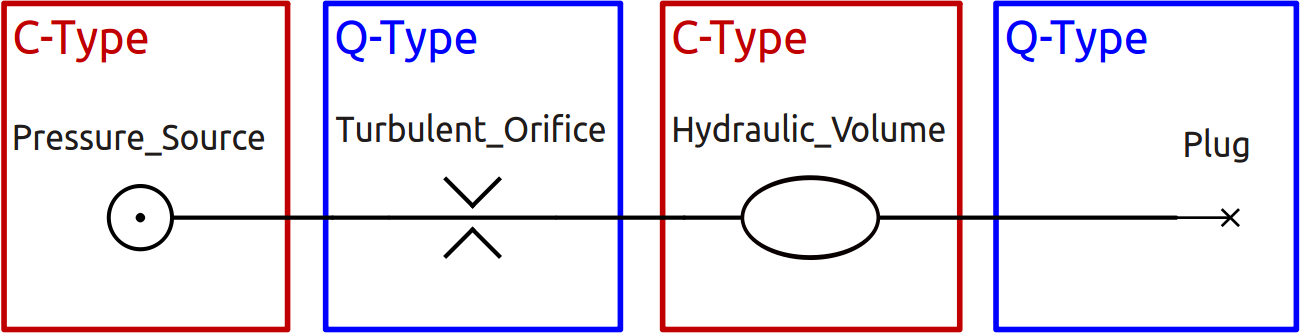
\includegraphics[width=1.0\linewidth]{gfx/cqs_startvalues/simplecqsystem.png}
\caption{A simple example of how C- and Q-type components must be connected in pairs}
\label{fig:simplecqsystem}
\end{figure}

\section{Sign Convention in C-type and Q-type Components}
In Hopsan there is currently no reference coordinate system, that is, there is no pre-defined common \enquote{positive direction} for all components.
You could say that the simulation is \enquote{zero-dimensional}.
If you are not aware of how \enquote{positive direction} is defined for a component it may be difficult to interpret the simulation results.

\todo[inline]{mention sama data in c and q ports (node behind)}

We must recognise two different variable types, \enquote{Flow} and \enquote{Effort} variables, in the power ports on the C- or Q-type components. 
They are listed for some node types in table~\ref{tab:floweffortvariables}.

\begin{table}[ht]
 \begin{tabular}{l|l|l}
   NodeType & Flow Variable & Effort Variable\\
   \hline
   Hydraulic & Flow \textbf{q} & Pressure \textbf{p} \\
   Linear Mechanic & Velocity \textbf{v} & Force \textbf{F}\\
   Rotational Mechanics & Angular Velocity $\dot{\theta}$ & Torque \textbf{T}\\
   Electric & Current \textbf{I} & Voltage \textbf{V}
 \end{tabular}
 \caption{Flow and effort variables for different node types}
 \label{tab:floweffortvariables}
\end{table}

\subsection*{Q-type Components}
The \enquote{positve direction} of the \enquote{flow} variables and their integrals are defined outwards from the power ports on Q-type component as shown in figure~\ref{fig:}
In the example system shown in figure~\ref{fig:simplecqsystem}, the flow travels from the right  to the left into the volume until it is filled.
If you plot the flow \textbf{q} from the left and right port of the (Q-type) orifice, figure~\ref{fig:} they will be the same but inverted around zero.
Since there is no \enquote{direction} defined, there is no way for Hopsan to know what \enquote{positive direction} you expect.
%Luckily you can set the \textit{plotscale} to -1 if you wish, to invert the plot.

If you plot the \enquote{effort} variable, pressure \textbf{p}, figure~\ref{fig:} you will see that it is positive on both sides.
In Hydraulic, Pneumatic or Electric simulations the pressure or voltage can never be lower then 0. 
You can never have a negative effort variable in these cases.
This is, however, not the case in Mechanical simulations, this is covered in more detail in section~\ref{sec:}.

\subsection*{C-type Components}
The C-type components are the TLM elements in Hopsan. 
They calculate the \enquote{Charcteristic Imedance} and \enquote{Wave variable}. 
You will likely not want to plot and examine these variables unless for debugging purposes but it is usefull to know that the \textbf{wave variable} represent the \enquote{effort variable} and that the \textbf{Characteristic Impedance} should always be a positive value.

The \enquote{positive direction} for power ports on C-type components are defined inwards into the port, as shown in figure~\ref{fig:}. 
The fact that c-type and q-type components have their \enquote{positive directions} defined like this means that you can always connect them to each other even if you invert the direction. 
This should only be relevant for component authors, however.


\section*{Sign convention in signal components}
In Hopsan there are also Signal-type Components that are not based on the TLM method.
The can be used to model a causal signal flow as shown in figure~\ref{fig:}.
Signal-type components and some C-type and Q-type components have input- and output-variable ports, sometimes refered to as read and write ports.
Theses ports do not have a direction, they simply represent scalar values and may be positive or negative.

\section*{Default Start Values}
Before a simulation starts you can set default start values in the ports and components to control the starting state for the simulation.
Start values are accessed through the component properties dialogue.
Default start values are written to the ports \textbf{before} the initialization is run.
This means that they may be overwritten by new values that are calculated during the initialization.
The resulting values in the ports after initialization are called the \textbf{initial values}, if no initialization of a particular port variable has been made, then the default start value will remain.
Some start values, will affect the initialization of internal component states.


\subsection*{Input variables}

\subsection*{Output variables}

\subsection*{Power Port variables}

The simplest example is the Signal-type \enquote{Constants} component which only has the output-variable default start value as a parameter. 

\todo[inline]{Here we must mention a warning that some components may seem to have startvalues that are ignored, you need to read the code to know for sure}


For input variables \textbf{defaulStartValues} determine 


\section*{Special case, mechanical components}




\end{document}